\documentclass[xcolor=svgnames,aspectratio=169]{beamer} 
\usetheme{metropolis}
\usefonttheme{professionalfonts}
\setbeamertemplate{theorems}[numbered]
\usepackage{luatexja}
\usepackage{luatexja-fontspec}
\usepackage{newtxtext}                     
\usepackage{amsthm} 
\usepackage{graphicx}
\usepackage{xcolor}
\usepackage{tcolorbox}
\usepackage{tikz}
\everymath{\displaystyle}
\usepackage{bm}
\usepackage{bbm}
\usepackage{lmodern}
\newcommand{\indep}{\mathop{\perp\!\!\!\!\perp}}
\newcommand{\R}{\mathbb{R}} 
\newcommand{\N}{\mathbb{N}} 
\newcommand{\Z}{\mathbb{Z}} 
\newcommand{\Q}{\mathbb{Q}} 
\newcommand{\C}{\mathbb{C}}
\newcommand{\E}{\mathbb{E}}

\begin{document} 

\title{Matrix Completion Methods for Causal Panel Data Models \\ \small{Susan Athey et al. (2021), JASA}}
\author{Naoki Eguchi}          
\institute{Faculty of Medicine, Kyoto University} 
\date{2025.6.25 ミクロ計量経済学}

\begin{frame}                  
    \titlepage                     
\end{frame}

\section{Introduction}

\begin{frame}{Today's Agenda ; Keyword : Imputation}
    \begin{itemize}
        \item
    \end{itemize}
\end{frame}

\begin{frame}{Imputation}
    \begin{itemize}
        \item As many panel data methods, we want to know ATT : $\E[Y_{it}(1)-Y_{it}(0)|W_i=1]$.
        \item Thus, it boils down to estimate (impute) the counterfactual $Y_{it}(0)$.
        \begin{itemize}
            \item Horizontal : Under unconfoundedness, we can impute counterfactual PO using observed outcomes for control units.
            \item Vertical : By SCM, we can also impute it using weighted average outcomes for control units with most predictive weights trained with pre-treatment datas.
        \end{itemize}
        \begin{figure}
            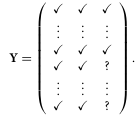
\includegraphics[width=0.5\textwidth, height=0.4\textheight, keepaspectratio]{Horizontal.png} \ 
            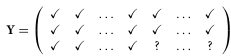
\includegraphics[width=0.5\textwidth, height=0.5\textheight, keepaspectratio]{Vertical.png}
        \end{figure}
    \end{itemize}
\end{frame}

\begin{frame}{Xu (2024): Counterfactual estimation}
    \begin{itemize}
        \item functional form: 
        $
        Y_{it}(0)=f(\mathbf{X_{it}})+h(\mathbf{U_{it}})+\epsilon_{it}
        $ \\
        \rightarrow No anticipation, carryover, feedback, LDV
        \item strict exogeneity:
        $
        \forall i,j\in\{1,\dots,N\},\ \forall s,t\in\{1,\dots,T\}, \epsilon_{it}\ \indep\ \{D_{js}, \mathbf{X_{js}}, \mathbf{U_{js}}\}
        $
        \begin{figure}
            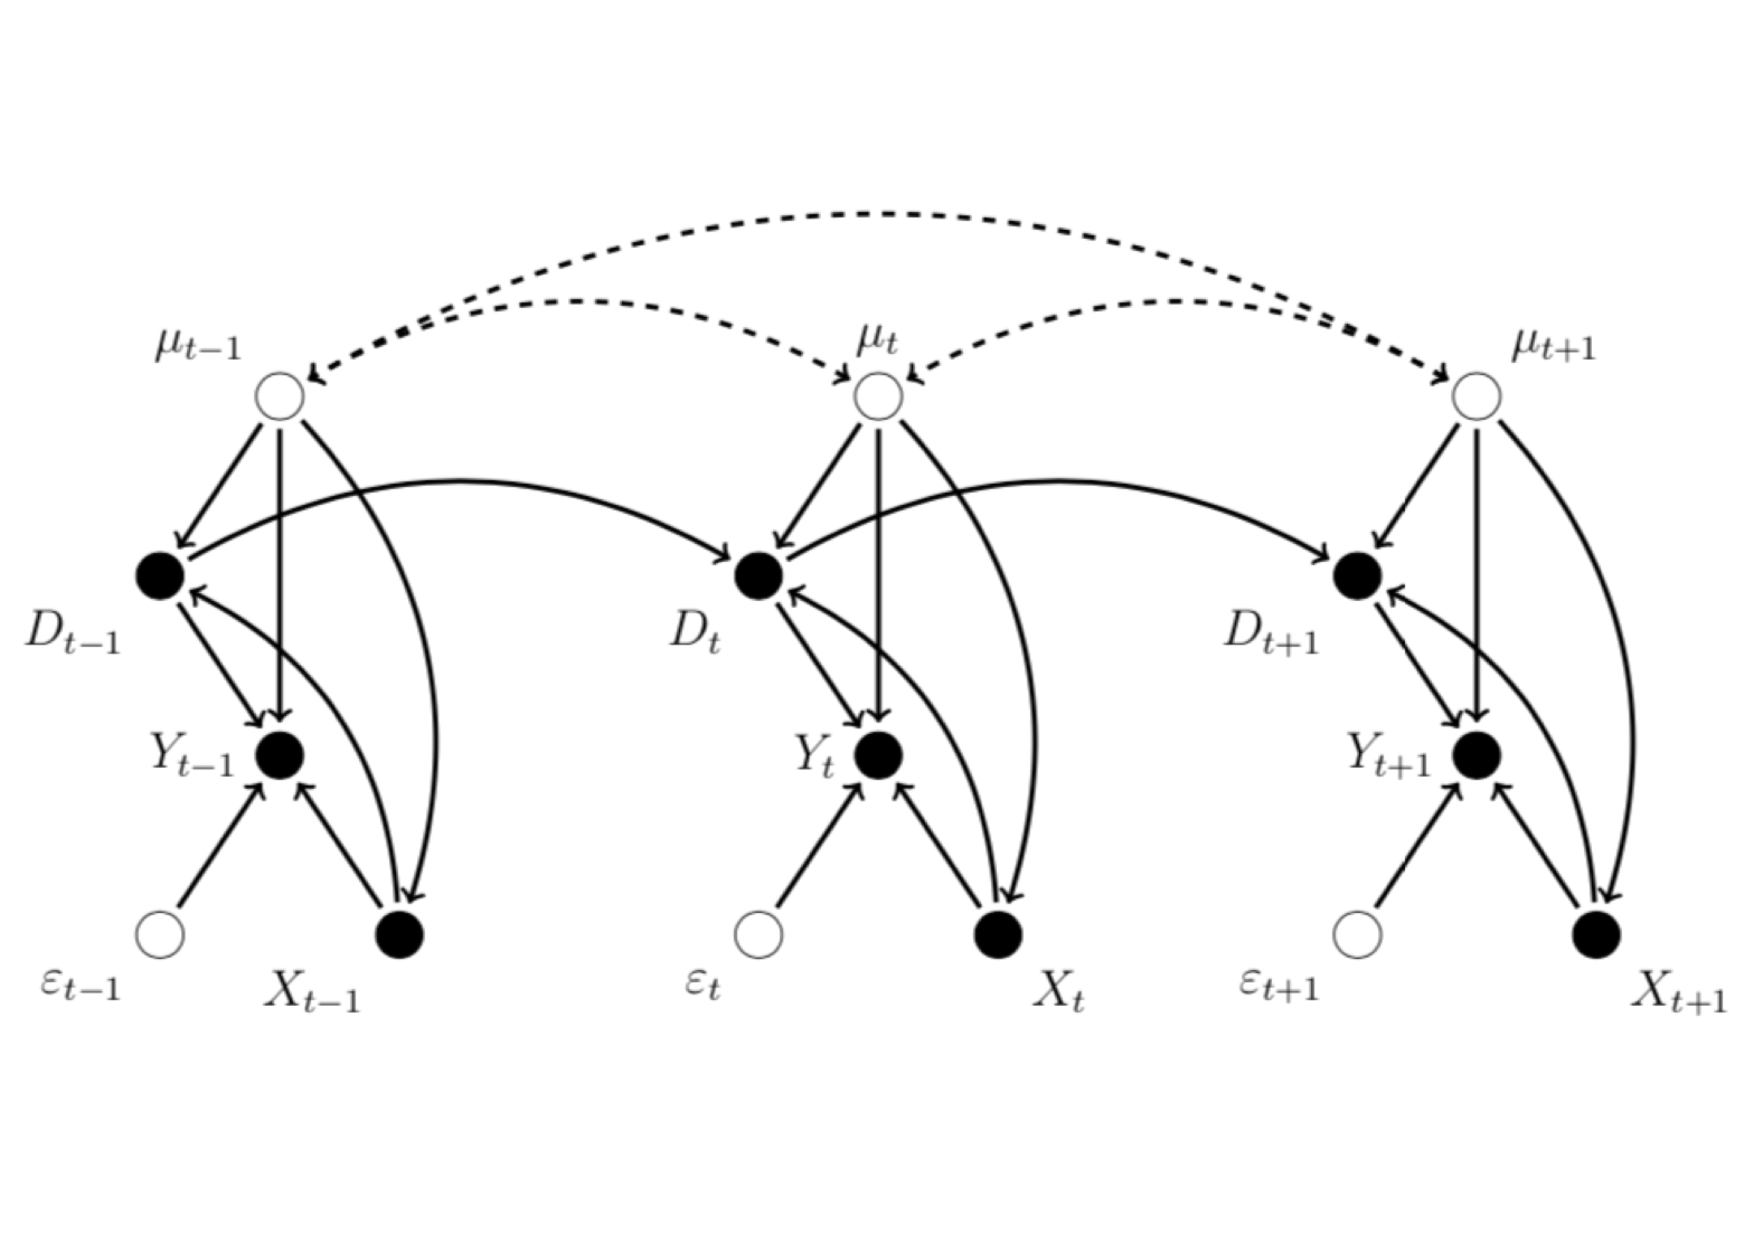
\includegraphics[width=\textwidth, height=0.4\textheight, keepaspectratio]{Xu_DAG.pdf}
        \end{figure}
        \item low-dimensional decomposition:
        $
        h(\mathbf{U_{it}})=\{L_{it}\}, \mathrm{rank}(\mathbf{L}_{N\times T}) \ll \min\{N,T\}
        $

        →The rank (= number of factors) is \alert{FIXED !!}
    \end{itemize}
\end{frame}

\section{Set Up}

\begin{frame}{Notation and Estimand}
    \begin{itemize}
        \item Consider a setting with $N$ units observed over $T$ periods characterized by a binary treatment $W_{it}$ and hence two POs $Y_{it}(1), Y_{it}(0)$.
        \begin{itemize}
            \item $\mathbf{X}\in\R^{N\times P} \ , \  \mathbf{Z}\in\R^{T\times Q}$ : observe (unit / time)-specific covariance matrix
        \end{itemize}
        \item Estimand : $\mathbf{Y} = \{Y_{it}(0)\footnote{以降は簡単のため,$Y_{it}(0)=Y_{it}$ とし,“(0)” を省略して表記する.}\}
        =
        \begin{pmatrix}
Y_{11}(0) & \cdots & Y_{1T}(0) \\
\vdots & \ddots & \vdots \\
Y_{N1}(0) & \cdots & Y_{NT}(0)
\end{pmatrix}$ (← Matrix!!)
        \item $W_{it}=
        \begin{cases}
            1 & \text{if} \ (i,t)\in \mathcal{M} \\ 0 & \text{if} \ (i,t) \in\mathcal{O} 
        \end{cases}$
    \end{itemize}
\end{frame}

\begin{frame}{Patterns of data matrix}
    \begin{itemize}
        \item Ordinary case (rich data wrt. units and times)
        \begin{figure}
            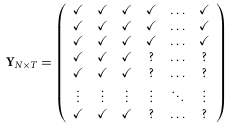
\includegraphics[width=\textwidth, height=0.35\textheight, keepaspectratio]{Ordinary.png}
        \end{figure}
        \item Staggered adoption
        \begin{figure}
            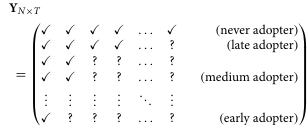
\includegraphics[width=\textwidth, height=0.35\textheight, keepaspectratio]{Staggered_adoption.png}
        \end{figure}
    \end{itemize}
\end{frame}

\begin{frame}{Horizontal regression and unconfoundedness : thin matrix ($N\gg T$)}
    \begin{figure}
            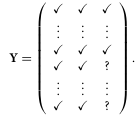
\includegraphics[width=0.5\textwidth, height=0.4\textheight, keepaspectratio]{Horizontal.png} 
        \end{figure}
    \begin{enumerate}
        \item Regress the last period outcome on the lagged outcomes. (among untreated)
        \item Predict the missing POs using the estimated regression.
        \[
        \forall (i,T)\in\mathcal{M} , \ \hat{Y}_{iT}=\hat{\beta}_0+\sum_{t=1}^{T-1}\hat{\beta}_tY_{it}, \ \text{where} \ \ \hat{\beta}=\arg\min_{\beta} \sum_{i:(i,T) \in \mathcal{O} }(Y_{iT}-\beta_0-\sum_{t=1}^{T-1}\beta_tY_{it})^2.
        \]
    \end{enumerate}
    →Nonparametrically, 
\end{frame}

\begin{frame}{Vertical regression and synthesis control : fat matrix ($T\gg N$)}
    \begin{figure}
            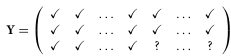
\includegraphics[width=0.5\textwidth, height=0.5\textheight, keepaspectratio]{Vertical.png}
    \end{figure}
    \begin{enumerate}
        \item Regress the outcomes for treated unit prior to the treatment on the outcomes for the control units in the same periods.
        \item Predct the missing POs using the estimated regression.
        \[
        \forall (N,t)\in\mathcal{M} , \ \hat{Y}_{Nt}=\hat{\gamma}_0+\sum_{i=1}^{N-1}\hat{\gamma}_iY_{it}, \ \text{where} \ \ \hat{\gamma}=\arg\min_{\gamma} \sum_{t:(N,t) \in \mathcal{O} }(Y_{Nt}-\gamma_0-\sum_{i=1}^{N-1}\gamma_iY_{it})^2.
        \]
    \end{enumerate}
    →Vertical regression is generalization of ADH(2010) in that it relaxes two restrictions :
    \begin{itemize}
        \item the coefficients $\hat{\gamma}$ are nonnegative. (Interpretability ; What is a negative weight?)
        \item the intercept in this regression is $0$. (This is seen to be plausible in recent literatures.)
    \end{itemize}
\end{frame}

\section{Matrix Completion}

\begin{frame}{Model}
    \begin{itemize}
        \item Under no covariates, we model the $N\times T$ matrix of complete matrix $\mathbf{Y}$ as
        \[
        \mathbf{Y}=\mathbf{L^*}+\mathbf{\epsilon}, \ \text{where} \ \ \E[\mathbf{\epsilon}|\mathbf{L^*}]=0.
        \]
    \begin{tcolorbox}[colframe=lightgray,title=Assumption 1]
        \begin{itemize}
            \item $\mathbf{\epsilon}$ is independent of $\mathbf{L^*}$ (strict exogeneity)
            \item The element of $\mathbf{\epsilon}$ are $\sigma-sub-Gaussian$ and independent each other.
            $\Leftrightarrow \forall t, \ \E[\exp (t\epsilon)]\leq \exp (\frac{\sigma^2t^2}{2}).$
        \end{itemize}
    \end{tcolorbox}
        \item The goal is to estimate the matrix $\mathbf{L^*}$. (low-rank assumption) 
    
        →Note that two types\footnote{これら以外にもInteractive fixed effectといったあらゆるfactorを"少数まで"許容する} of fixed effects are included.
    \end{itemize}
\end{frame}

\begin{frame}{MC-NNM (Matrix Completion with Nuclear Norm Minimization) estimator}
    \begin{itemize}
        \item MC-NNM estimator for $\mathbf{L^*}$ is given by $\mathbf{\hat{L}}+\hat{\Gamma}\mathbf{1}_T' + \mathbf{1}_N\hat{\Delta}'$
        \[
        (\mathbf{\hat{L}}, \hat{\Gamma}, \hat{\Delta})=\arg \min_{\mathbf{L},\Gamma,\Delta} 
        \{
            \frac{1}{|\mathcal{O} |}  ||\mathbf{P_{\mathcal{O} }}({\mathbf{Y}-\mathbf{L}-\Gamma}\mathbf{1}_T'-\mathbf{1}_N\Delta')||_F^2+\lambda||\mathbf{L}||_*
        \}
        \]
        \begin{itemize}
            \item $\Gamma\in\R^N$ : unit-varying (and time-fixed) effect (individual effect)
            \item $\Delta\in\R^T$ : time-varying (and unit-fixed) effect (time effect) 
            \item matrix indicator function : $\mathbf{P_{\mathcal{O} }}(\mathbf{A})=
            \begin{cases}
                A_{it} & \text{if} \ (i,t)\in\mathcal{O} \\ 0 & \text{if} \ (i,t) \notin \mathcal{O}  
            \end{cases}$ \ (NA is regarded as $0$)
            \item Frobenius norm : $||\mathbf{A}||_F^2=\sum_{i=1}^N\sum_{t=1}^T A_{it}^2$ \ (行列版のmean squared errorを計算している)
        \end{itemize}
        \item Regularization term $\lambda||L||_*$ leads to \alert{the low rank of $\mathbf{L}$}. \\
        → minimize $\lambda||L||_*$ $\Leftrightarrow $ the sparsity of Singular value $\sigma_i(\mathbf{L})(>0)$ $\Leftrightarrow $ low rank of $\mathbf{L}$
    \end{itemize}
\end{frame}

\begin{frame}
    \begin{itemize}
        \item \textbf{Fact 1.} (Singular value decomposition) \textit{Every real matrix $L\in\R^N\times \R^T$ can be decomposed using a onthogonal matrix $\mathbf{S}\in \R^N\times \R^{\min(N,T)},\mathbf{R}\in\R^T\times \R^{\min(N,T)}$ by}
        \[
        \mathbf{L}=\mathbf{S}\mathbf{\Sigma}\mathbf{R'}, \text{where} \ \mathbf{\Sigma}=\text{diag}(\sigma_1,\dots\sigma_{\min(N,T)}), \mathbf{S'S=I_{\min(N,T)}=R'R}
        \]
        \item \textbf{Fact 2.} \textit{The number of non-zero singular value = rank $\mathbf{L}$}
        \begin{itemize}
            \item Nuclear norm : $||L||_*=\sum_{i=1}^{\min(N,T)} \sigma_i(\mathbf{L})$ \\
            → minimize $\lambda||L||_*$ $\Leftrightarrow $ the sparsity of Singular value $\sigma_i(\mathbf{L})(>0)$ $\Leftrightarrow $ low rank of $\mathbf{L}$
        \end{itemize}
        \item Since the rank of $\mathbf{L}$ corresponds to \alert{the number of factor}, this assumption of low rank is quite plausible. 
        \item Although the law rank matrix CAN include two fixed effects, these "strong" factors are separately estimated for improving the quality of the practical imputations.
    \end{itemize}
\end{frame}

\begin{frame}{Algorithm for calculating $\hat{\mathbf{L}}$}
    \begin{itemize}
        \item For simplicity, assume that there are no fixed effects. (only estimate $\mathbf{L}$)
        \item \textbf{Fact 3.} \textit{For $\mathbf{A=S\Sigma R}$, the minimizer is obtained analytically.}
        \[
        \mathbf{S\tilde{\Sigma}R^\mathsf{T}}=\arg\min_{\mathbf{A}}\{\frac{1}{2}||\mathbf{L-A}||_F^2+\lambda||\mathbf{A}||_*\}, \text{where} \ \tilde{\Sigma}=\text{diag}(\{\max(\sigma_i(\mathbf{A})-\lambda,0)\}_i)
        \]
        → You can see elements with a small singular value (=weak factor) will be vanished.
        \item We perform this minimization over and over until the matrix converges.
        \begin{itemize}
            \item Define $\text{shrink}_{\lambda}(\mathbf{A})=\mathbf{S\tilde{\Sigma}R^\mathsf{T}}$ and start with the initial choice $\mathbf{L_1}(\lambda, \mathcal{O})=\mathbf{P}_\mathcal{O} (\mathbf{Y})$ (The missing starts with $0$.)
            \[
            \mathbf{L}_{k+1}(\lambda,\mathcal{O} )=\text{shrink}_{\frac{\lambda|\mathcal{O} |}{2}}\{\mathbf{P}_{\mathcal{O} }(\mathbf{Y})+\mathbf{P}_{\mathcal{O} }^\mathsf{T}(\mathbf{L}_k(\lambda,\mathcal{O} ))\}
            \]
            \item $\mathbf{P_{\mathcal{O} }}(\mathbf{A})=
            \begin{cases}
                A_{it} & \text{if} \ (i,t)\in\mathcal{O} \\ 0 & \text{if} \ (i,t) \notin \mathcal{O}  
            \end{cases}$ \ , \quad $\mathbf{P_{\mathcal{O} }^\mathsf{T}}(\mathbf{A})=
            \begin{cases}
                0 & \text{if} \ (i,t)\in\mathcal{O} \\ A_{it} & \text{if} \ (i,t) \notin \mathcal{O}  
            \end{cases}$
            \item The limiting matrix $\hat{\mathbf{L}}(\lambda,\mathcal{O} )=\lim_{k\to \infty} \mathbf{L}_k(\lambda,\mathcal{O} )$ is MC-NNM estimator given $\lambda$.
        \end{itemize}
    \end{itemize}
\end{frame}

\begin{frame}
    \begin{itemize}
        \item For the case with fixed effects,  
    \end{itemize}
\end{frame}

\begin{frame}{Inference : CV and CI}
    \begin{itemize}
        \item The optimal value of $\lambda$ is selected through \alert{cross-validation}.
        \begin{itemize}
            \item 
        \end{itemize}
        \item The theory of asymptotic distribution of $\mathbf{L^*}-\mathbf{\hat{L}}$ to construct CI has not yet developed.
        \item Instead, using resampling method, we see the fluctulation of the imputed matrix and construct CI like premutation methods in ADH-synthetic control method.
    \end{itemize}
\end{frame}

\section{The relationship with horizontal and vertical regressions}

\begin{frame}
    \begin{itemize}
        \item Let the estimand $\mathbf{Y}$ partition as $
        \begin{pmatrix} \mathbf{Y_0} & \mathbf{y_1} \\ \mathbf{y_2}' & ? \end{pmatrix}$, \\ where $\mathbf{Y_0}\in\R^{N-1}\times \R^{T-1}, \mathbf{y_1}\in\R^{N-1}, \mathbf{y_2}\in\R^{T-1}$.
        \item For a given positive integer $R$, define an $N\times R$ matrix $\mathbf{A}$, an $T\times R$ matrix $\mathbf{B}$, a $N$-dim. vector $\gamma$ and a $R$-dim. vector $\delta$, then, the objective function w.r.t. MSE is
        \[
        Q(\mathbf{Y}; R, \mathbf{A}, \mathbf{B}, \gamma, \delta)=\frac{1}{|\mathcal{O} |} ||\mathbf{P_{\mathcal{O} }}({\mathbb{Y}-\mathbf{AB'}-\gamma}\mathbf{1}_T'-\mathbf{1}_N\delta')||_F^2
        \]
    \end{itemize}
\end{frame}

\begin{frame}{MC-NNM estimator}
    \begin{itemize}
        \item Nuclear norm matrix completion
        \begin{align*}
        (R_\lambda^{\mathrm{mc\text{-}nnm}},\,
         \mathbf{A}_\lambda^{\mathrm{mc\text{-}nnm}},\,
         \mathbf{B}_\lambda^{\mathrm{mc\text{-}nnm}},\,
         \gamma_\lambda^{\mathrm{mc\text{-}nnm}},\,
         \delta_\lambda^{\mathrm{mc\text{-}nnm}})& \\
        = \arg\min_{R,A,B,\gamma,\delta}
           \Bigl\{Q(\mathbf{Y};R,\mathbf{A},\mathbf{B},\gamma,\delta)
        &+\frac{\lambda}{2}\|\mathbf{A}\|_F^2
           +\frac{\lambda}{2}\|\mathbf{B}\|_F^2\Bigr\}.
        \end{align*}
        \item \textbf{Fact 3.} $\|\mathbf{L}\|_*
        = \min_{\mathbf{A},\mathbf{B}:\,\mathbf{L}=\mathbf{A}\mathbf{B}'}
          \frac{1}{2}\bigl(\|\mathbf{A}\|_F^2 + \|\mathbf{B}\|_F^2\bigr).$
  \end{itemize}
\end{frame}

\begin{frame}{Horizontal regression (thin matrix, $N>T$)}
  \begin{itemize}
    \item Horizontal regression estimator
      \begin{align*}
        &(R^{hr},\,\mathbf{A}^{hr},\,\mathbf{B}^{hr},\,\gamma^{hr},\,\delta^{hr})
        = \arg\min_{R,A,B,\gamma,\delta}
           Q\bigl(\mathbf{Y};R,\mathbf{A},\mathbf{B},\gamma,\delta\bigr),\\
        &\text{subject to}\quad
        R = T-1,\quad
        \mathbf{A} = \begin{pmatrix}\mathbf{Y}_0 \\ y_2^\top\end{pmatrix},\quad
        \gamma = 0,\quad
        \delta_1 = \cdots = \delta_{T-1} = 0.
      \end{align*}
    \item The solution for $\mathbf{B}$ is
    \[
      \mathbf{B}^{hr\top}
      = \begin{pmatrix} E_{T-1} & \hat\beta \end{pmatrix},
      \quad
      (\hat\beta,\hat\delta_T)
      = \arg\min_{\beta,\delta_T}
        \sum_{i=1}^{N-1}
        \bigl(Y_{iT} - \delta_T - \sum_{t=1}^{T-1}\beta_t\,Y_{it}\bigr)^2.
    \]
  \end{itemize}
\end{frame}


\begin{frame}
    \begin{itemize}
        \item Vertical regression, defined if $T>N$ : fat matrix
    \end{itemize}
\end{frame}

\begin{frame}{Another methods}
    \begin{figure}[h]
  \centering
  \begin{minipage}{0.43\columnwidth}
    \centering
    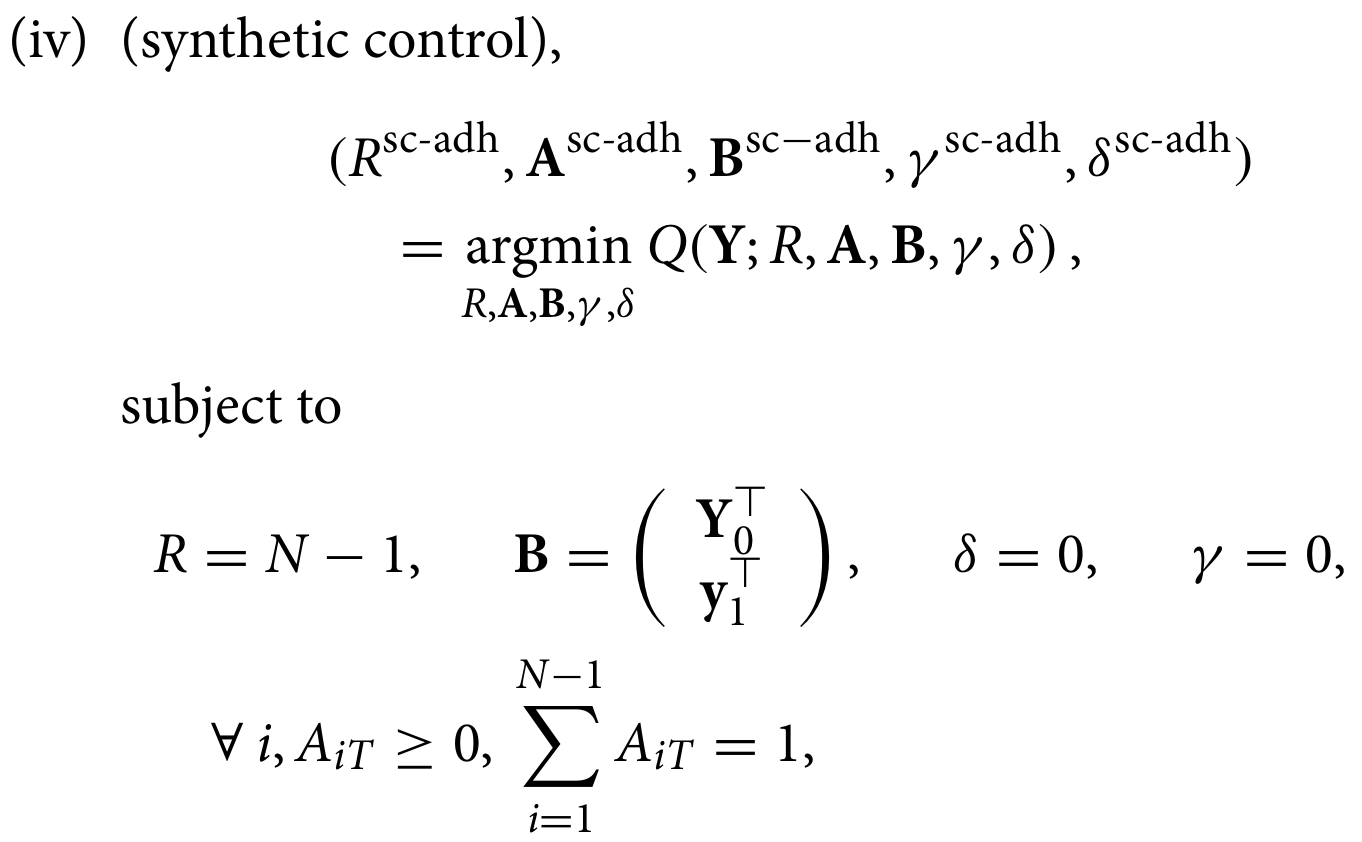
\includegraphics[width=0.95\textwidth, height=0.95\textheight, keepaspectratio]{SC.png}
  \end{minipage}
  \hspace{5mm}
  \begin{minipage}{0.43\columnwidth}
    \centering
    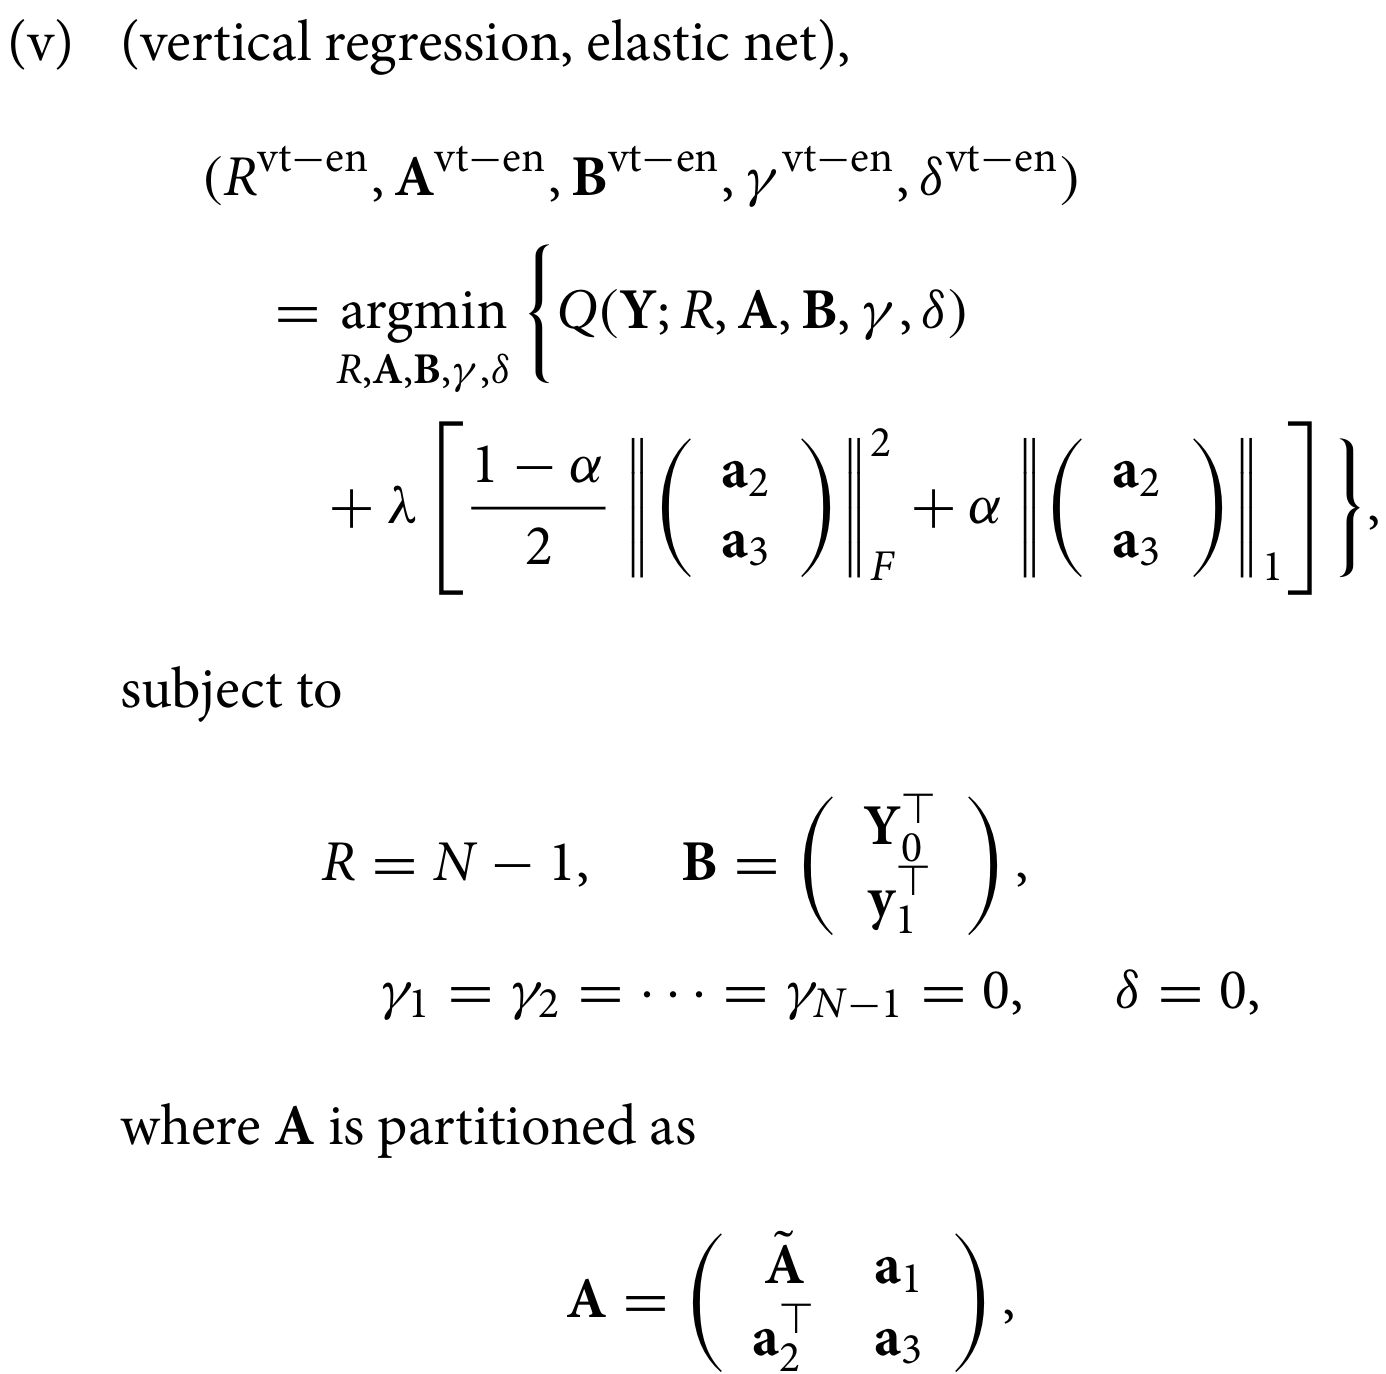
\includegraphics[width=0.95\textwidth, height=0.95\textheight, keepaspectratio]{Vt_EN.png}
  \end{minipage}
  \end{figure}
\end{frame}

\section{Theoritical Bounds \\ for the Estimation Error}

\begin{frame}{Estimation error}
    \begin{itemize}
        \item 
    \end{itemize}
\end{frame}

\section{Two illustrations}

\begin{frame}{Comparing each method}
    \begin{itemize}
        \item In a real data matrix $\mathbf{Y}$ where \alert{no units is treated}, we choose units as "hypothetical treated" units (=regard as missing) and aim to predict (impute) their value. \\
        → Technically, compare the average root-mean-squared-error(RMSE) to assess which of the algorithm generally perform well.
        \item The compared estimators (algorithms) are as follows.
        \begin{itemize}
            \item DiD : 2回差分によりcounterfactualを補完する
            \item VT-EN : elastics netでvertical regression functionを作り、その推定値で補完
            \item HR-EN : elastics netでhorizontal regression functionを作り、その推定値で補完
            \item SC-ADH : classical approach to construct "synthetic control".
            \item MC-NNM : 本日の主役
        \end{itemize}
    \end{itemize}
\end{frame}

\begin{frame}{ADH(2010): California smoking data}
    \begin{itemize}
        \item $N=38, T=31$
        \begin{itemize}
            \item Simultaneous adoption : Let randomly selected $N_t=8$ units "treated" in period $T_0+1$.
            \item Staggered adoption : Let randomly selected $N_t=35$ units "treated" in some periods after period $T$.
            \begin{figure}
            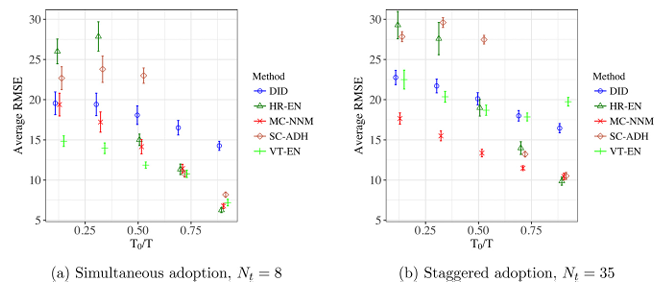
\includegraphics[width=0.7\textwidth, height=0.4\textheight, keepaspectratio]{ADH.png}
            \end{figure}
        \end{itemize}
        \item (a) : VT-EN performs well on the whole, DiD is poor.
        \item (b) : MC-NNM is superior (large sample is favorable!), and VT-EN is generally poor.
    \end{itemize}
\end{frame}

\begin{frame}{Stock market data}
    \begin{itemize}
        \item 
    \end{itemize}
\end{frame}

\section{Final marks}

\begin{frame}{Summary and Conclusion}
    \begin{itemize}
        \item Matrix completion is a imputing method for the missing $Y_{it}(0)$ where $(i,t)\in \mathcal{M}$.
        \item MC-NNM estimator is the generalization of many estimators such as DiD, ADH-SC, vertical or horizontal (penalized) regression , and interactive fixed effect model.
        \item The critical differnce with previus estimators is that MC-NNM \alert{holistically restricts} the factors by regularization with sparsity (Intrinsic factor vs Explicit factor)
        \item Practically, this estimator performs well with large $N$ and $T$, and allows for a relatively large number of factors.
        \item 
    \end{itemize}
\end{frame}

\section{References}

\begin{frame}{References}
    \begin{itemize}
        \item Susan Athey, Mohsen Bayati, Nikolay Doudchenko, Guido Imbens, and Khashayar Khosravi (2021), \textit{Matrix Completion Methods for Causal Panel Data Models}, Journal of the American Statistical Association.
        \item Licheng Liu, Ye Wang, and Yiqing Xu (2024), \textit{A Practical Guide to Counterfactual Estimators for Causal Inference with Time-Series Cross-Sectional Data},  American Journal of Political Science.
        \item Jungjun Choi and Ming Yuan(2024), \textit{Matrix Completion When Missing Is Not at Random and Its Applications in Causal Panel Data Models}, Journal of the American Statistical Association.
        \item Martin J. Wainwright (2019), \textit{High-Dimensional Statistics}, Cambridge University Press. (mainly Chapter 10)
        \item 冨岡亮太 (2015), スパース性に基づく機械学習, 講談社.
        \item 川口康平,澤田真行 (2024), 因果推論の計量経済学,日本評論社.
    \end{itemize}
\end{frame}

\end{document}